\section{Resultados}\label{sec:resultados}
\subsection{Soluciones 1D y verificación del código}
Con los datos de la Tabla~\ref{tab:datos}, la Formulación II converge a $Q_1=6.9405\,\Qs$, $Q_2=5.0595\,\Qs$ y $H_J=101.5937$ m ($y_J=1.5937$ m), es decir $\varphi=0.4216$, igual para los cinco ángulos. La Formulación I da, en cambio, un reparto que crece con el ángulo (Tabla~\ref{tab:f1}), con $\lambda=0.75$ y $\mu=0.50$. La diferencia de nivel entre ramales que exigiría el flujo ideal, $(y_1-y_2)/y$, crece de $0.45\pc$ en $30^\circ$ a $15.9\pc$ en $90^\circ$ y $32.3\pc$ en $120^\circ$.

\begin{table}[H]
\centering\small
\caption{Fracción al ramal 2 según la Formulación I.}\label{tab:f1}
\begin{tabular}{lccccc}
\toprule
$\alpha$ ($^\circ$) & 30 & 45 & 60 & 90 & 120\\\midrule
$\varphi_{\mathrm I}=Q_2/Q_0$ & 0.4063 & 0.4353 & 0.4779 & 0.6025 & 0.7845\\\bottomrule
\end{tabular}
\Fuente{Elaboración propia, Newton--Raphson sobre \eqref{eq:f1}.}
\end{table}

La convergencia de Newton--Raphson para la Formulación II se detalla en la Tabla~\ref{tab:iter}: el residuo cae de $1.2\times10^{-1}$ a $2\times10^{-15}$ en cuatro iteraciones, con el comportamiento cuadrático esperado cerca de la raíz. La Figura~\ref{fig:redes} muestra las redes de flujo de la Formulación I para $30^\circ$, $60^\circ$, $90^\circ$ y $120^\circ$ con la geometría de la Fase I del cuaderno ($\lambda=1$, $\mu=0.5$), distinta de la del caso nominal.

\begin{table}[H]
\centering\small
\caption{Historial de Newton--Raphson, Formulación II, caso nominal.}\label{tab:iter}
\begin{tabular}{rrrrr}
\toprule
Iteración & $Q_1$ ($\Qs$) & $Q_2$ ($\Qs$) & $H_J$ (m) & $\|\mathbf F\|_\infty$\\\midrule
0 & 8.823406 & 3.176594 & 101.490000 & $1.247\times10^{-1}$\\
1 & 6.717514 & 5.282486 & 101.568979 & $3.577\times10^{-2}$\\
2 & 6.936867 & 5.063133 & 101.593352 & $5.227\times10^{-4}$\\
3 & 6.940494 & 5.059506 & 101.593677 & $1.326\times10^{-7}$\\
4 & 6.940494 & 5.059506 & 101.593678 & $2.186\times10^{-15}$\\\bottomrule
\end{tabular}
\Fuente{Elaboración propia, \path{codigo/newton_bifurcacion.py}.}
\end{table}

\begin{figure}[H]
\centering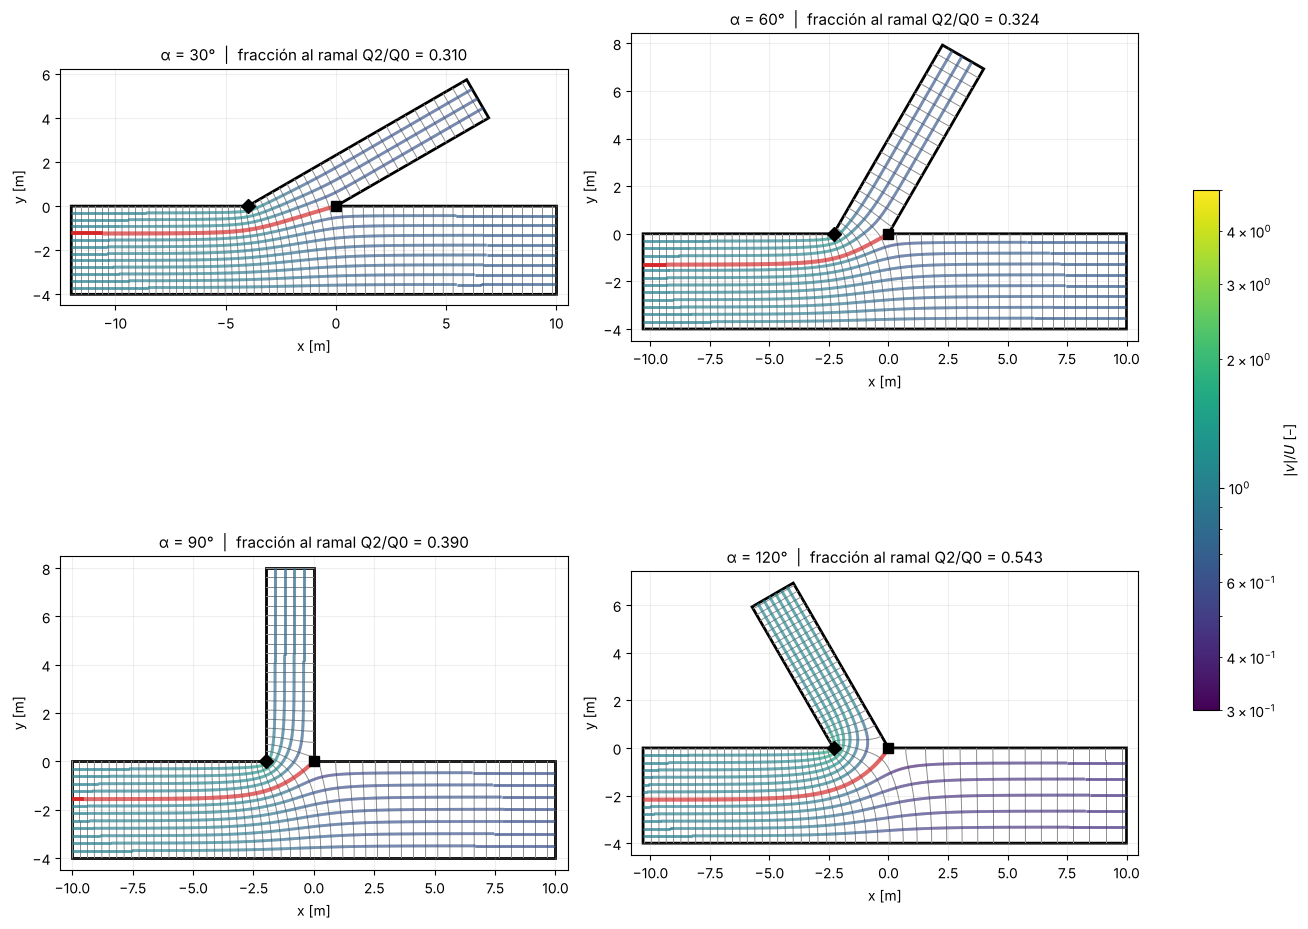
\includegraphics[width=0.92\linewidth]{3.png}
\caption{Redes de flujo de la Formulación I (potencial ideal con tapa rígida) para varios ángulos; la fracción al ramal se indica sobre cada panel.}\label{fig:redes}
\Fuente{Elaboración propia con el cuaderno de la Fase I. Los repartos indicados (0.310, 0.324, 0.390 y 0.543) corresponden a $\lambda=1$ y $\mu=0.5$ y se reprodujeron con Newton--Raphson sobre \eqref{eq:f1}; los de la Tabla~\ref{tab:f1} corresponden a $\lambda=0.75$ y $\mu=0.50$.}
\end{figure}

La Tabla~\ref{tab:verif} resume las pruebas. El benchmark de la red de ocho canales \emph{no se reproduce}: la reconstrucción difiere hasta 33.3\pc (10.5 $\Qs$) de los valores tabulados, y varios calados de esa red se excluyeron por inconsistencias internas. Se reporta como prueba no superada; no se afirma que el código de la red esté validado.

\begin{table}[H]
\centering\small
\caption{Pruebas de verificación.}\label{tab:verif}
\begin{tabular}{>{\raggedright\arraybackslash}p{0.34\linewidth}>{\raggedright\arraybackslash}p{0.34\linewidth}>{\raggedright\arraybackslash}p{0.14\linewidth}}
\toprule
Prueba & Resultado & Estado\\\midrule
Simetría, ramales idénticos & $Q_1=Q_2=2.0000\,\Qs$; error 0 (tolerancia $10^{-10}$) & Cumple\\
Conservación de masa, caso nominal & $Q_1+Q_2-Q_0=0.0000$ & Cumple\\
Hoja 1D del 90° vs. Formulación II & Coincide ($Q_1=6.9405$, $Q_2=5.0595$) & Cumple\\
Hoja de Milne-Thomson vs. Formulación I & Diferencia máx. $|\Delta\varphi|=4.5\times10^{-7}$ & Cumple\\
Red de ocho canales (Chaudhry) & Diferencia relativa máx. 33.3\pc & No cumple\\\bottomrule
\end{tabular}
\end{table}

\subsection{Sensibilidad del reparto}
La Figura~\ref{fig:elast} muestra las elasticidades de $\varphi$ para los 13 parámetros, evaluadas en las configuraciones del conjunto exploratorio inicial (calados de salida del 2D de entonces). Dominan los calados de control ($|E|\approx0.8$ a $1.3$, con signo opuesto entre ramales), los anchos de fondo ($|E|\approx0.75$ a $0.96$) y la rugosidad ($|E|\approx0.5$). El caudal total, las longitudes y el coeficiente local tienen efecto pequeño ($|E|\leq0.26$; $|E(K)|\approx0.03$). La incertidumbre postulada produce $\sigma_\varphi=0.031$ a $0.036$ en la aproximación lineal y $0.033$ a $0.037$ en Monte Carlo, con diferencias de $-0.4$ a $+7.6\pc$ entre ambos métodos, de modo que la linealización es adecuada.

\begin{figure}[H]
\centering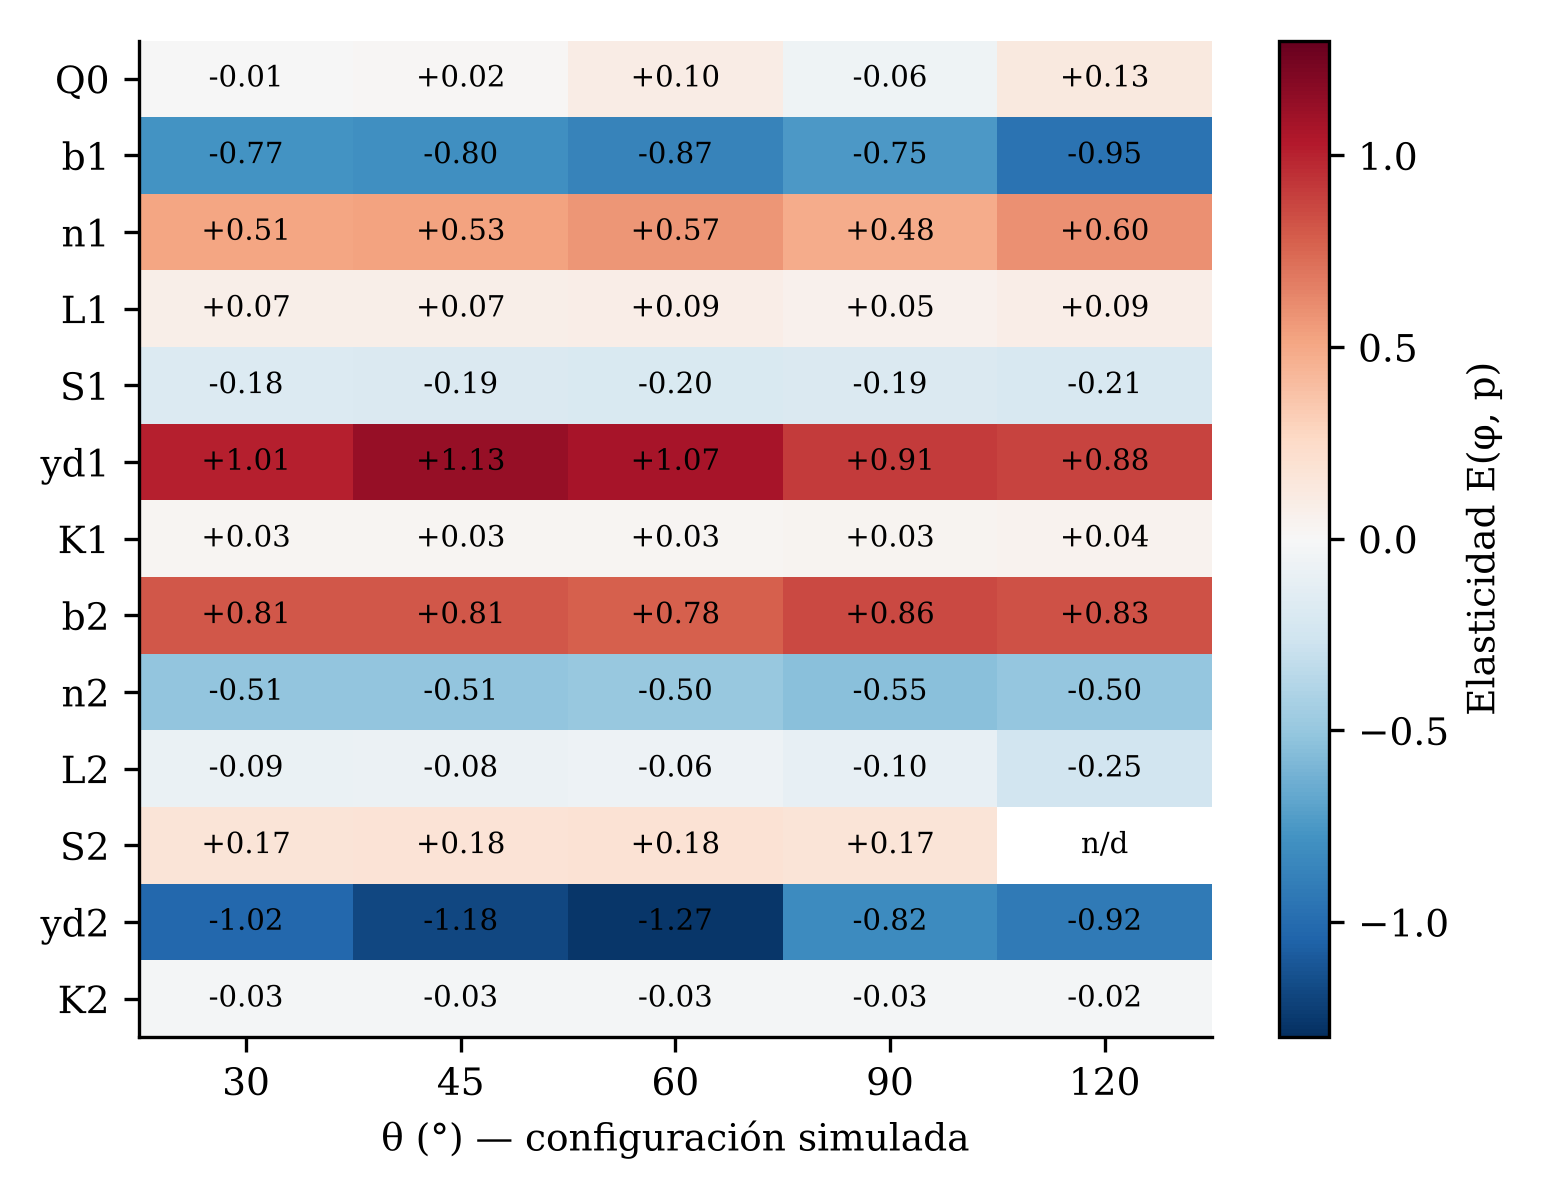
\includegraphics[width=0.62\linewidth]{fig_elasticidad.png}
\caption{Elasticidades de $\varphi$ por ángulo (configuraciones del conjunto exploratorio inicial). Para $120^\circ$, $S_2=0$ y la elasticidad de $S_2$ no está definida.}\label{fig:elast}
\Fuente{Elaboración propia, cuaderno de la Fase IV.}
\end{figure}

\subsection{Sensibilidad de la Formulación II a $K$ y a $n$}
Dos parámetros se barren aparte porque son los que se discuten al comparar con el 2D (Tabla~\ref{tab:barrido}). La pérdida local $K$ casi no mueve el reparto: de $K=0$ a $2.4$, $\varphi$ pasa de $0.4232$ a $0.4142$ (diferencia $0.009$). En cambio, \emph{reducir} la rugosidad en ambos ramales \emph{aumenta} $\varphi$ ($0.4741$ con $n$ al 72\pc del nominal), de modo que una resistencia efectiva menor en el 2D no puede explicar un reparto menor.

\begin{table}[H]
\centering\small
\caption{Reparto de la Formulación II al variar $K$ (con $n$ nominal) y al escalar $n$ en ambos ramales (con $K=0.2$).}\label{tab:barrido}
\begin{tabular}{lccccc}
\toprule
$K$ & 0 & 0.2 & 0.5 & 1 & 2.4\\
$\varphi_\mathrm{II}$ & 0.4232 & 0.4216 & 0.4198 & 0.4176 & 0.4142\\\midrule
$n/n_\mathrm{nom}$ & 1.00 & 0.93 & 0.86 & 0.72 & \\
$\varphi_\mathrm{II}$ & 0.4216 & 0.4314 & 0.4430 & 0.4741 & \\\bottomrule
\end{tabular}
\Fuente{Elaboración propia, \path{codigo/newton_bifurcacion.py} con los datos de la Tabla~\ref{tab:datos}.}
\end{table}

\subsection{Verificación del 2D en ramales rectos aislados}\label{sec:resverif}
Con SWE-EM y celda de 0.25 m el nivel simulado sigue el remanso 1D con diferencias de pocos centímetros, pero la resistencia efectiva depende de la malla: $n_\mathrm{eff}/n=0.93$, $0.86$ y $0.72$ para celdas de 0.50, 0.25 y 0.125 m, con el mismo valor en los dos ramales (Tabla~\ref{tab:neff}); aproximadamente $n_\mathrm{eff}/n\approx1-0.035/\Delta x$. En el ramal 2 del nudo a $30^\circ$ la tendencia con la malla es la contraria ($n_\mathrm{eff}$ de $0.0183$ a $0.0233$ al refinar), de modo que la geometría diagonal añade una resistencia propia del modelo.

\begin{table}[H]
\centering\small
\caption{Resistencia efectiva en ramales rectos aislados (SWE-EM).}\label{tab:neff}
\begin{tabular}{cc}
\toprule
Celda (m) & $n_\mathrm{eff}/n$\\\midrule
0.50 & 0.93\\
0.25 & 0.86\\
0.125 & 0.72\\\bottomrule
\end{tabular}
\Fuente{Elaboración propia con los resultados HDF de los ramales aislados.}
\end{table}

La corrección lineal \emph{no cumple} la comprobación (Tabla~\ref{tab:correccion}). Con $n$ de entrada $0.0174$ en el ramal 1 se obtiene $n_\mathrm{eff}=0.0143$ (objetivo $0.0150$) y un error máximo de nivel de $0.018$ m; con $0.0212$ en el ramal 2 se obtiene $0.0170$ (objetivo $0.0180$) y $0.041$ m. Los niveles siguen por debajo del 1D, es decir, aún falta resistencia: la respuesta del modelo a $n$ no es lineal ($n_\mathrm{eff}/n_\mathrm{entrada}$ baja de $0.86$ a $0.82$). Por eso la corrección se reporta solo como diagnóstico y no se aplicó a las corridas del nudo.

\begin{table}[H]
\centering\small
\caption{Prueba de corrección de $n$ (celda 0.25 m).}\label{tab:correccion}
\begin{tabular}{lccccc}
\toprule
Ramal & $n$ entrada & $n_\mathrm{eff}$ objetivo & $n_\mathrm{eff}$ obtenido & Error máx. de nivel (m) & Criterio ($\pm0.01$ m)\\\midrule
1 & 0.0174 & 0.0150 & 0.0143 & 0.018 & No cumple\\
2 & 0.0212 & 0.0180 & 0.0170 & 0.041 & No cumple\\\bottomrule
\end{tabular}
\Fuente{Elaboración propia con los resultados HDF de los ramales aislados (planes con $n$ corregido).}
\end{table}

\subsection{Control de calidad de las corridas del nudo}
Las cinco corridas con celda de 0.25 m cumplen los criterios de aceptación (Tabla~\ref{tab:cc}): error de volumen entre $2.7\times10^{-6}$ y $8.9\times10^{-3}\pc$, cierre de caudal $\leq0.009\pc$ y reparto idéntico entre los últimos 600 s y los 600 s previos. En $90^\circ$ el cálculo informa un error máximo de nivel de celda de 0.62 m en una celda aislada junto a la punta de la divisoria (a $x\approx-0.1$ m, $y\approx2.1$ m del nudo), sin efecto sobre el volumen ni sobre los caudales.

\begin{table}[H]
\centering\small
\caption{Control de calidad de las corridas SWE-EM con celda de 0.25 m.}\label{tab:cc}
\begin{tabular}{rcccc}
\toprule
$\theta$ ($^\circ$) & Celdas & Error de volumen (\%) & Cierre de caudal (\%) & $\varphi$ última 600 s / previa\\\midrule
30 & 20174 & $3.1\times10^{-6}$ & 0.000 & 0.3739 / 0.3739\\
45 & 23092 & $8.9\times10^{-3}$ & 0.009 & 0.3581 / 0.3581\\
60 & 20207 & $3.1\times10^{-6}$ & 0.000 & 0.3503 / 0.3503\\
90 & 24108 & $7.1\times10^{-4}$ & 0.001 & 0.3402 / 0.3402\\
120 & 20248 & $2.7\times10^{-6}$ & 0.000 & 0.3132 / 0.3132\\\bottomrule
\end{tabular}
\Fuente{Elaboración propia, resúmenes de cálculo y series de caudal de los planes HDF.}
\end{table}

\subsection{Reparto: contraste 1D--2D}
La Tabla~\ref{tab:reparto} y la Figura~\ref{fig:phitheta} contrastan las formulaciones con el 2D. El 2D da un reparto que \emph{decrece} con el ángulo, de $0.374$ a $0.313$. La Formulación I crece de $0.406$ a $0.785$: acierta en magnitud a $30^\circ$ ($+8.7\pc$) pero se aleja con el ángulo hasta $+150\pc$ a $120^\circ$, con tendencia opuesta. La Formulación II es constante en $0.4216$ y sobrestima $Q_2$ entre $+12.8$ y $+34.6\pc$, con un error que crece con $\theta$. Con el conjunto exploratorio SWE-ELM de 0.125 m, el reparto es $\approx0.41$ entre $30^\circ$ y $60^\circ$ y la II queda a $+2.2$ a $+2.9\pc$, pero a $90^\circ$ y $120^\circ$ la brecha sube a $+11.2$ y $+28.7\pc$.

\begin{table}[H]
\centering\small
\caption{Reparto $\varphi=Q_2/Q_0$ del 2D y de las formulaciones; $\varepsilon(Q_2)$ (\%) entre paréntesis.}\label{tab:reparto}
\begin{tabular}{rccccc}
\toprule
$\theta$ ($^\circ$) & 2D SWE-EM 0.25 m & Form. I & Form. II & 2D SWE-ELM 0.125 m & II vs. ELM\\\midrule
30 & 0.3739 & 0.4063 (+8.7) & 0.4216 (+12.8) & 0.4107 & (+2.7)\\
45 & 0.3581 & 0.4353 (+21.6) & 0.4216 (+17.7) & 0.4124 & (+2.2)\\
60 & 0.3503 & 0.4779 (+36.4) & 0.4216 (+20.4) & 0.4096 & (+2.9)\\
90 & 0.3402 & 0.6025 (+77.1) & 0.4216 (+23.9) & 0.3790 & (+11.2)\\
120 & 0.3132 & 0.7845 (+150.5) & 0.4216 (+34.6) & 0.3275 & (+28.7)\\\bottomrule
\end{tabular}
\Nota{En las columnas de las formulaciones, $\varepsilon(Q_2)$ se calcula respecto del 2D SWE-EM; la última columna, respecto del 2D SWE-ELM. SWE-ELM es exploratorio (Sección~\ref{sec:hecras}). Fuente: elaboración propia.}
\end{table}

\begin{figure}[H]
\centering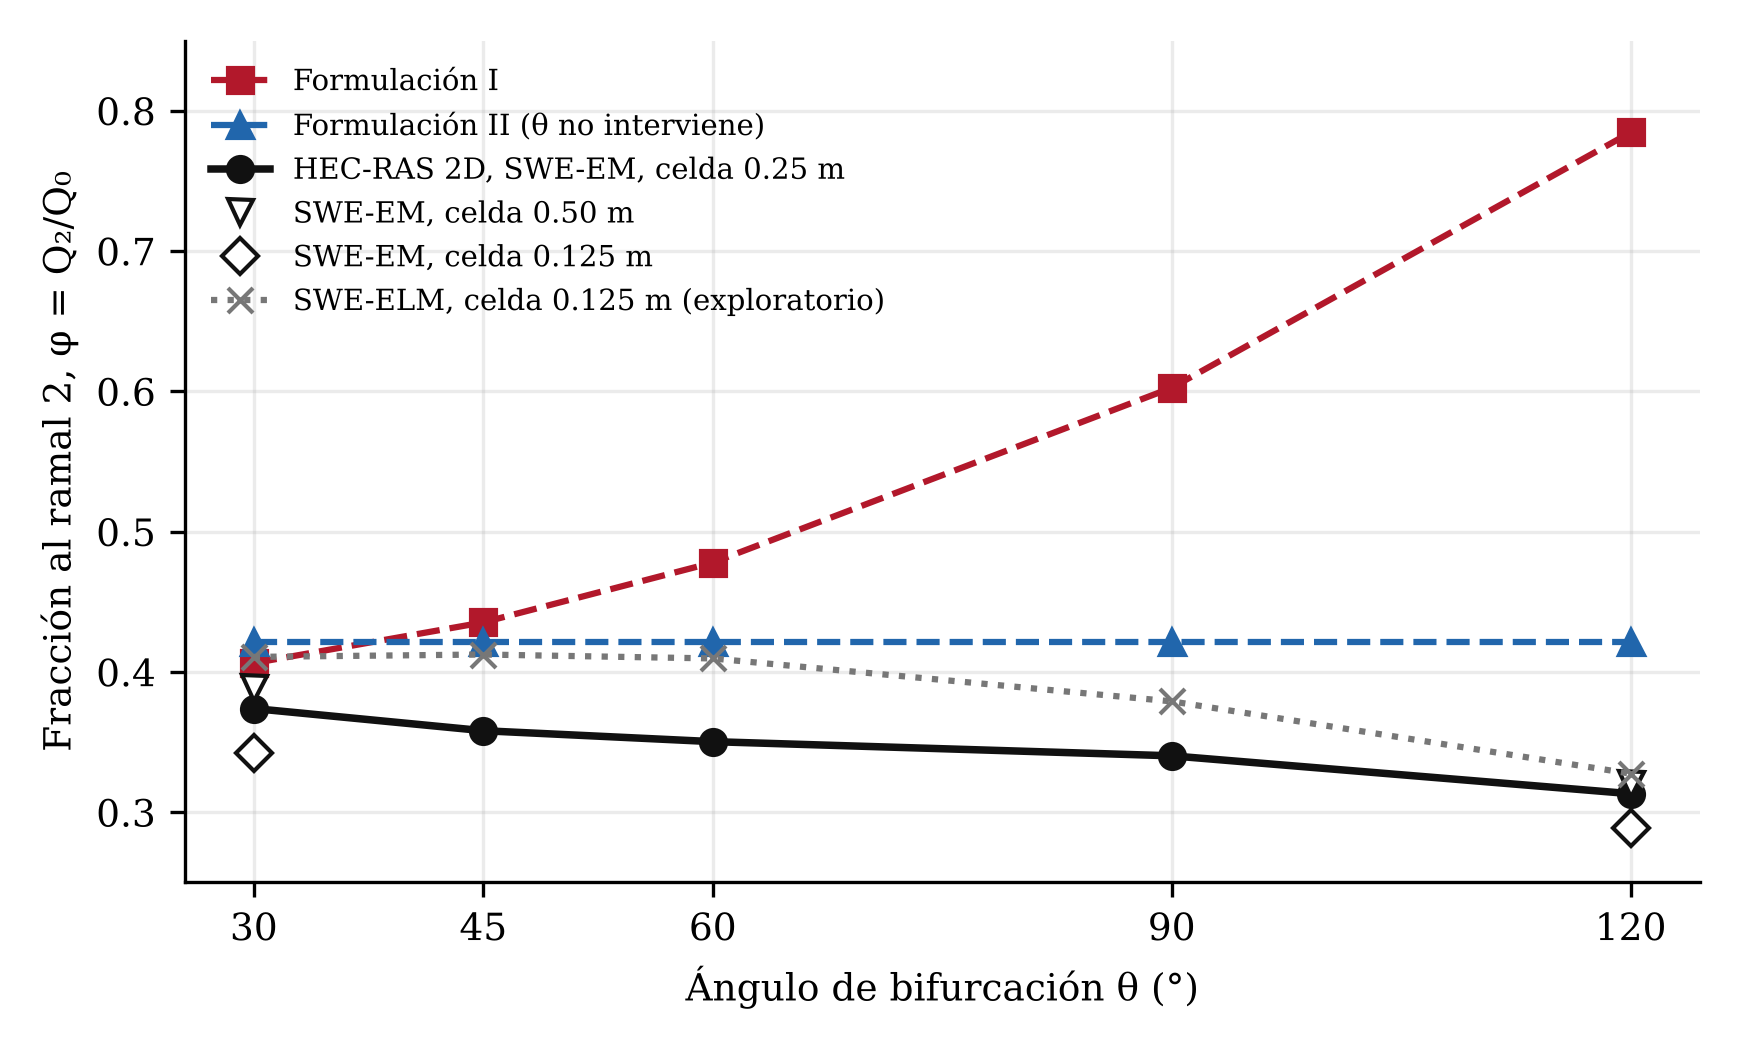
\includegraphics[width=0.78\linewidth]{fig_phi_theta.png}
\caption{Fracción al ramal 2 en función del ángulo. Los marcadores vacíos muestran la dispersión por malla del SWE-EM en 30° y 120°.}\label{fig:phitheta}
\Fuente{Elaboración propia (\path{datos/resultados_2d_v3.csv}, \path{datos/mallas_EM.csv}, \path{datos/mallas_ELM.csv}).}
\end{figure}

\subsection{Dependencia de la malla y de las ecuaciones}
En SWE-EM, $\varphi$ \emph{no converge} al refinar (Tabla~\ref{tab:mallas}, Figura~\ref{fig:malla}a): a $30^\circ$ baja de $0.389$ a $0.374$ y a $0.343$ para celdas de 0.50, 0.25 y 0.125 m, con diferencias crecientes ($0.015$ y $0.031$); a $120^\circ$ baja de $0.320$ a $0.313$ y a $0.289$. Como las diferencias crecen, no corresponde aplicar el GCI ni la extrapolación de Richardson. En cambio, refinar solo el nudo sobre la malla de 0.25 m cambia poco el resultado ($0.378$ y $0.379$ a $30^\circ$; $0.317$ y $0.316$ a $120^\circ$): la resolución local del nudo está convergida y la dependencia viene de la malla de los ramales y del canal, coherente con la pérdida de resistencia efectiva de la Sección~\ref{sec:resverif}. La corrida uniforme de 0.125 m en $120^\circ$ presenta un error de volumen mayor ($4.8\times10^{-3}\pc$) y un cierre de $0.09\pc$, todavía aceptables.

Con SWE-ELM (Figura~\ref{fig:malla}b) el reparto cambia menos con la malla entre 0.25 y 0.125 m ($\leq0.007$ en 30°, 45° y 60°), pero difiere del de SWE-EM en $0.04$ a $0.07$ a igual malla de 0.125 m.

\begin{table}[H]
\centering\small
\caption{Reparto $\varphi$ del 2D SWE-EM según la malla (30° y 120°).}\label{tab:mallas}
\begin{tabular}{llccc}
\toprule
$\theta$ ($^\circ$) & Malla & Celdas & $\varphi$ & Error de volumen (\%)\\\midrule
30 & uniforme 0.50 m & 5372 & 0.3888 & $1.7\times10^{-8}$\\
30 & uniforme 0.25 m & 20174 & 0.3739 & $3.1\times10^{-6}$\\
30 & uniforme 0.125 m & 88440 & 0.3425 & $3.0\times10^{-6}$\\
30 & 0.25 m + nudo 0.125 m & 23198 & 0.3778 & $3.1\times10^{-6}$\\
30 & 0.25 m + nudo 0.0625 m & 35239 & 0.3789 & $3.1\times10^{-6}$\\
120 & uniforme 0.50 m & 5884 & 0.3204 & $1.8\times10^{-6}$\\
120 & uniforme 0.25 m & 20248 & 0.3132 & $2.7\times10^{-6}$\\
120 & uniforme 0.125 m & 88770 & 0.2886 & $4.8\times10^{-3}$\\
120 & 0.25 m + nudo 0.125 m & 23459 & 0.3174 & $2.7\times10^{-6}$\\
120 & 0.25 m + nudo 0.0625 m & 36044 & 0.3159 & $2.7\times10^{-6}$\\\bottomrule
\end{tabular}
\Fuente{Elaboración propia, planes HDF.}
\end{table}

\begin{figure}[H]
\centering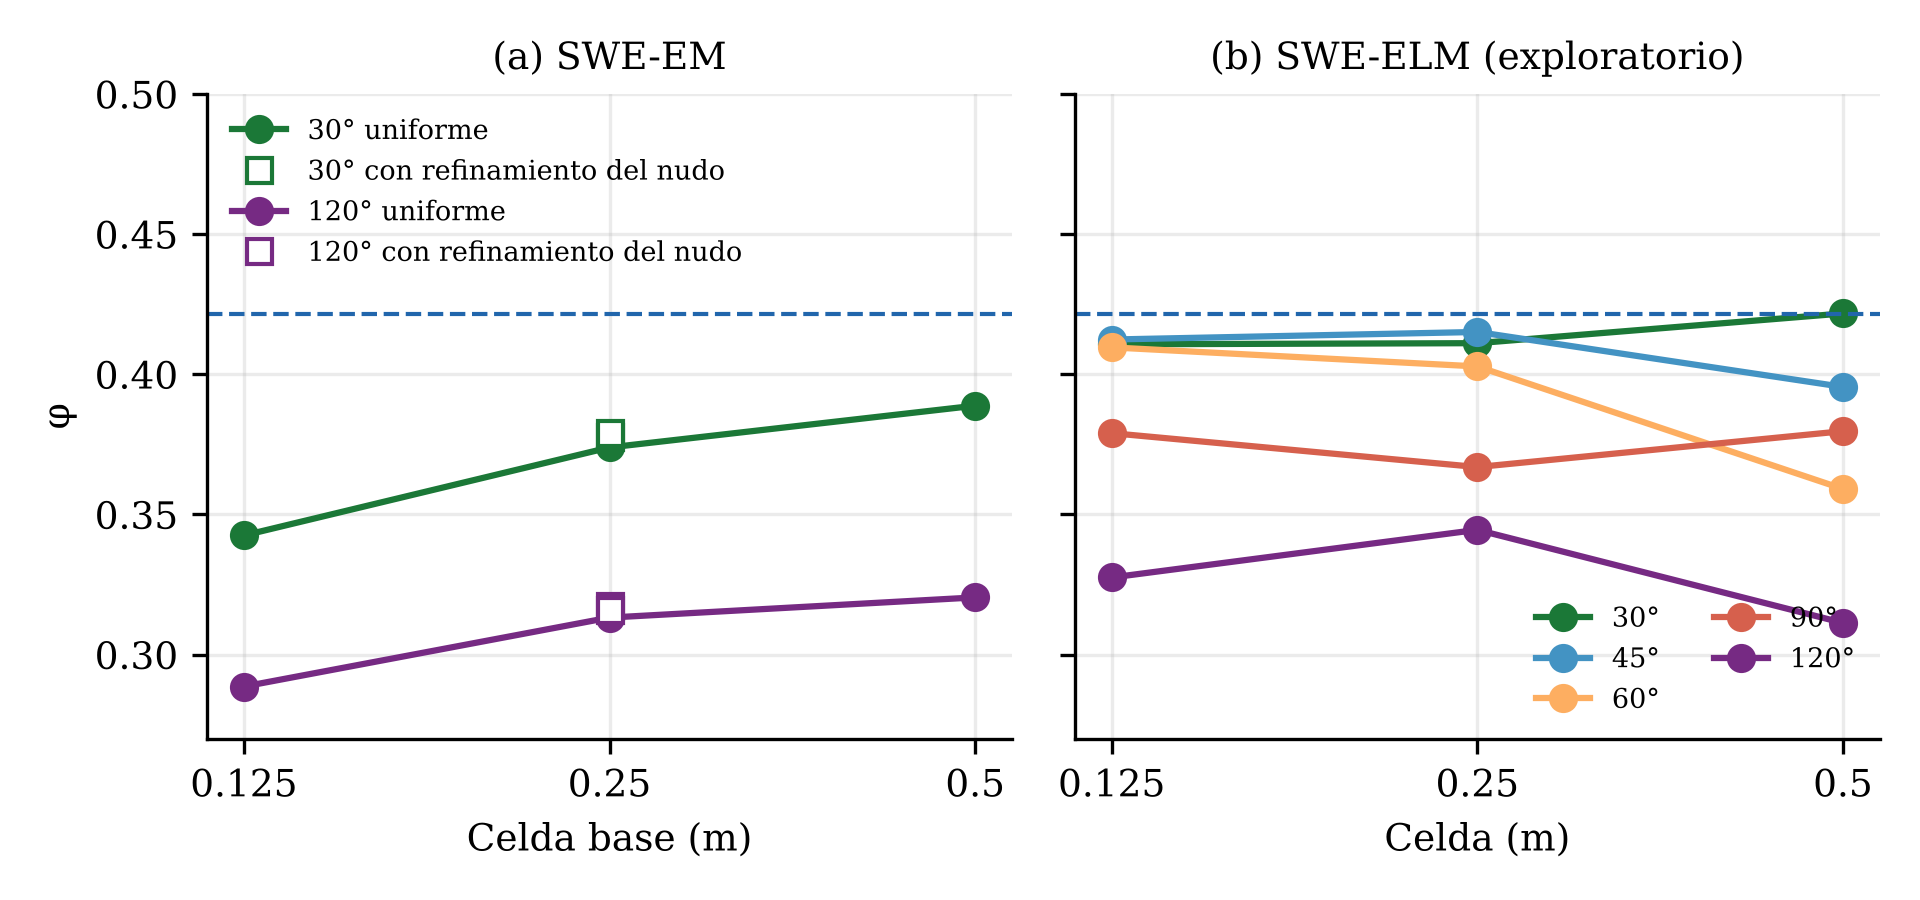
\includegraphics[width=0.92\linewidth]{fig_malla.png}
\caption{Reparto frente al tamaño de celda. (a) SWE-EM, 30° y 120°, con refinamiento local del nudo; (b) SWE-ELM, cinco ángulos. La línea discontinua es $\varphi_\mathrm{II}=0.4216$.}\label{fig:malla}
\Fuente{Elaboración propia.}
\end{figure}

\subsection{Energía en el nudo}
El balance de energía entre el canal principal y el inicio del ramal 2 en el 2D muestra una pérdida de carga que crece con el ángulo: unos $0.04$ m a $30^\circ$ y unos $0.22$ m a $120^\circ$, lo que corresponde a un coeficiente local efectivo $K_\mathrm{ef}\approx0.4$ a $0.5$ y $\approx2.4$ frente al $K=0.2$ fijo de la Formulación II (valores aproximados, malla de 0.25 m). Sin embargo, la Tabla~\ref{tab:barrido} indica que $\varphi_\mathrm{II}$ casi no responde a $K$ (de $0.4232$ a $0.4142$ para $K$ entre 0 y 2.4), de modo que un $K$ dependiente del ángulo no basta, por sí solo, para reproducir el descenso del reparto.
